\chapter{Analyse \& Design ( 25 \%)}
\label{chap:design}

Im vorhergehenden Kapitel wurden Ziele und Leistungskriterium
für das CI-System festgelegt.
Diese sollen nun auf konzeptueller Ebene umgesetzt werden.
Dazu wird zuerst ein Überblick des Gesamtkonzeptes gegeben.
Anschließend werden besondere Konzepte zur 
%XXX: continue


\section{Systemarchitektur}
\label{sec:design:sysarch}
Diese Sektion gibt Aufschluss über die Grobstruktur des CI-Systems auf logischer und physischer Ebene.

\subsection{logisch}

\begin{figure}[ht]
  \centering
  \label{fig:grob-layout-komponenten-logisch}
  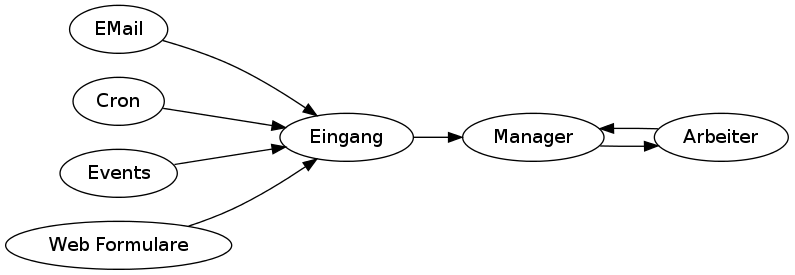
\includegraphics[width=\textwidth]{imageinput/grob-layout-komponenten-logisch.png}
  \caption{\"Ubersicht ber Systemkomponenten - logisch}
\end{figure}


Die erste wichtige Komponente ist der Eingang,
in ihm gehen Aufträge aus verschiedensten Quellen ein.
Nach dem sie validiert wurden, werden die Aufträge an
die zweite wichtige Komponente, den Manager, weitergegeben.
Dort werden sie vorbereitet und entsprechend der Build-Matrix Arbeitspakete erstellt.
Nun treten Manager und Arbeiter in eine Interaktion,
um zu bestimmen welcher Arbeiter das Eigentliche Arbeitspaket bearbeitet.
Anschließend werden die Arbeitspakete von den jeweilig designierten Arbeitern abgefertigt.

%XXX: more


\subsection{physisch}

\begin{figure}[ht] 
  \centering
  \label{fig:grob-layout-komponenten}
  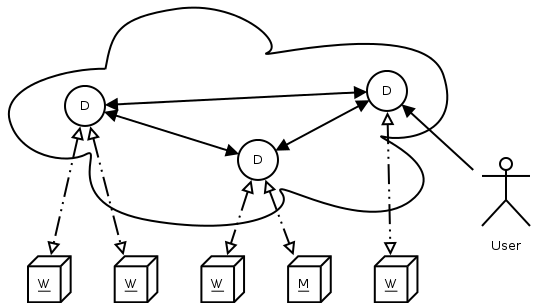
\includegraphics[width=\textwidth]{imageinput/grob-layout-komponenten.png}
  \caption{Übersicht über Systemkomponenten - physisch}
\end{figure}

Der physische Aufbau unterscheidet sich stark von den bisher dagewesenen CI-Systemen.
Grund ist der Fokus auf die verteilte Datenbank, direkte Kommunikation
wird der Interaktion mit einer verteilten Datenbank weichen.

Das System besteht somit aus Komponenten welche alle als Clients einer verteilten Datenbank operieren.
Die Abbildung~\ref{fig:grob-layout-komponenten} zweigt die Struktur.
Nennenswert ist dabei die Bindung einer Komponente and bestimmte Datenbank-knoten,
dies dient der Kontrolle der Lokalität und wird später noch vorgestellte Verfahrensweisen unterstützen.

%XXX more

\section{Datenschema}


\begin{figure}[ht] 
  \centering
  \label{fig:datenstrukturen}
  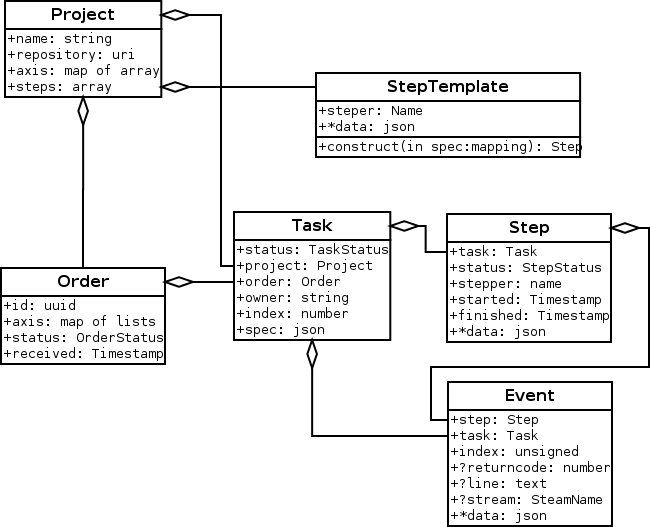
\includegraphics[width=\textwidth]{imageinput/datenstrukturen-step-templates.png}
  \caption{Grundlegende Datenstrukturen}
\end{figure}

Das grundlegende Datenschema, in Abbildung~\ref{fig:datenstrukturen} als UML Klassendiagramm dargestellt,
beschreibt die Daten des Kernsystems und einige ihrer Interaktionen.

Die wichtigsten Datentypen sind dabei Projekt, Auftrag (Order),
Arbeitspaket (Task) und Arbeitsschritt (Step).

\subsubsection{Projekt}

Das Projekt beinhaltet neben dem Namen auch alle Informationen,
die später für das Erstellen von Arbeitspaketen sowie
die Ausführung einer Integration benötigt werden.
Dazu gehört das Quellcode-repository (repo), von dem später
die Quelltexte für das dem Test unterworfenen Projekt bezogen werden.
Weiterhin beinhaltet es die Build-Achsen,
welche die Wertebereiche der einzelnen Ebenen der Build-Matrix
beschreiben.

\subsubsection{Arbeitsschritt Templates}

Der mitunter wichtigste Teil eines Projektes ist jedoch die Beschreibung der Arbeitsschritte als Templates.
Die Darstellung als Template ist dabei bewusst gewählt,
sie ermöglicht es jedem Arbeitspaket speziell konfigurierte Arbeitsschritte zur Verfügung zu stellen.
Außerdem bewirkt die erneute Speicherung in der Datenbank,
das Bearbeiten der Schritte eines Projektes keinen Einfluss auf bereits erstellte Arbeitspakete hat.
Zudem stellen die extra Objekte auch einen Anschlusspunk für die Datensammlung dar.
Die Methode \textit{construct} des Templates dient dazu,
einen Arbeitsschritt, angereichert mit einer entsprechenden Konfiguration, zurückzugeben.

\subsubsection{Auftrag}

Ein Auftrag beinhaltet grundsätzlich eine Referenz auf das zugehörige Projekt,
außerdem beinhaltet er Überschreibungen/Zusätze für die Build-Achsen,
dies Ermöglicht es sowohl in den Achsen eingeschränkte,
als auch erweiterte Aufträge zu erstellen.
Diese werden später genauer erklärt.
Zusätzlich beinhaltet der Auftrag einen Status, dieser beinhaltet den aktuellen Stand der Bearbeitung.

\subsubsection{Arbeitspaket}
%XXX: eventuell projekt hier nicht referenzieren
Ein Arbeitspaket beinhaltet neben Referenzen zu dem Projekt und dem Auftrag,
seine Spezifikation. Diese gibt die Ausbildung aller Build-Achsen für dieses Paket an.
des weiteren beinhaltet es den Index, dieser gibt die Numerische Position in der Build-Matrix an.
Auch ein Arbeitspaket hat einen Status, welcher den aktuellen Bearbeitung-stand zum Ausdruck bringt.
Zudem bestimmt das Feld ``Owner'' den Arbeiter, welcher das Arbeitspaket letztendlich bearbeiten wird.

\subsubsection{Arbeitsschritt}

Ein Arbeitsschritt referenziert das zugehörige Arbeitspaket.
Neben den Zeitpunkten für Anfang und Ende seiner Ausführung,
benennt er im Feld ``stepper'' um welche Art von Arbeitsschritt es sich handelt.
Das Feld ``status'' gibt Auskunft über den aktuellen Stand der Bearbeitung.
Das Feld ``data'' soll weitere dynamische Informationen zum Ausdruck bringen,
die bei der Ausführung genutzt werden.

%XXX: dies dient \ldots


\subsubsection{Event}
%XXX referenz auf task?

Das Event bringt Datensammlung zur Laufzeit zum Ausdruck.
Neben den Referenzen für den Arbeitsschritt und das Arbeitspaket,
beinhaltet es eine Indexnummer und einen Timestamp.
Die Indexnummer ist eine aufsteigende Zahl
und gibt den Events eines bestimmten Arbeitsschritts eine feste eindeutige Reihenfolge.
Der Timestamp gibt den Events eine zeitliche Ordnung (welche jedoch nicht eindeutig ist).


Zusätzlich zu diesen Basisdaten, beinhaltet ein Event beliebige weitere optionale Felder.
Einige mögliche (und ihre Datentypen) sind:

\begin{description}
    \dhitem[returncode: Number] Rückgabe-wert eines Prozesses bei seiner Beendigung.
    \dhitem[line: Text] Textzeile eines Datenstromes der Ausgabe
    \dhitem[lineno: Number] Zugeh. Zeilennummer
    \dhitem[stream: Name] Zugeh. Name des Datenstromes
    \dhitem[start: Name] Mitteilung über den Start eines best. Vorganges
    \dhitem[end: Name] Mitteilung über den Abschluss eines best. Vorganges
\end{description}




\section{Logik der Komponenten}

Diese Sektion behandelt die grundlegende Logik  der Einzelteile des Systems,
sie bilden die Bausteine für das Gesamtsystem.

%XXX MORE

\subsection{Auftragsannahme}

Der Auftragsannahme lässt sich grob in 2 Abschnitte einteilen.
Zuerst geht ein Auftrag ein, was je nach Methode in mehrere Schritte beinhalten kann,
danach wird er überprüft und damit angenommen oder abgelehnt.


\begin{figure}[ht]
  \centering
  \label{fig:lebenszyklus-auftrag-eingang}
  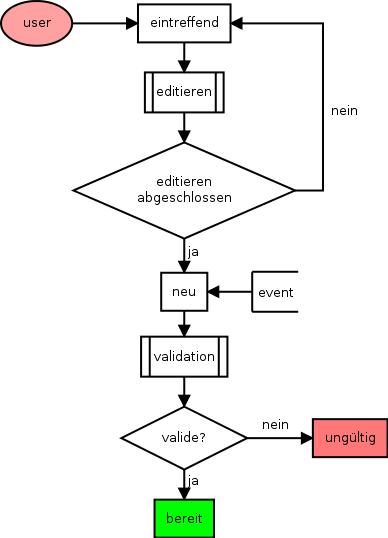
\includegraphics[height=5in]{imageinput/lebenszyklus-auftrag-eingang.png}
  \caption{Auftragsannahme: Flussdiagramm}
\end{figure}


\subsubsection{Eingang}

Auftragseingang gestaltet sich in der Praxis vielseitig.
Da nicht alle Quellen direkt einen fertigen Auftrag generieren können,
beginnt ein Auftrag im Zustand eingehend, sind schließlich alle Daten zusammengekommen,
so wird der Eingang festgehalten und der Auftrag wird vom System weiterverarbeitet.

%XXX Quellen betrachten``
Betrachtet werden die Anforderungen für die Quellen
\begin{description}
    \dhitem[EMail]
        Eingang per EMail kann in 2 Formen erfolgen,
        zum einen kann der gesamte Auftrag ein einer einzigen EMail enthalten sein.
        Zum anderen kann sich der Auftrag über mehr als eine EMail erstrecken.
        Beispiel hierfür sind z.B. Mercurial Patchbombs \cite{mercurial:patchbomb}.
        Ist ein Auftrag fertiggestellt, so ist eine Antwort-email hilfreich.
        Wichtig ist, dass EMails Unbekannter auf keinen Fall
        akzeptiert werden sollten.
    \dhitem[Mailingliste]
        Eingang per Mailingliste ist dem Eingang per Email sehr ähnlich,
        Haupt-unterschied ist, dass anstelle einer privaten Korrespondenz
        ein öffentliches Forum genutzt wird. Dabei sollen auch EMails Unbekannter 
        bearbeitet werden können.
        Ein bekanntes Beispiel für eine Mailingliste mit Patches
        ist die Mercurial Mailingliste \cite{mercurial:mailingliste}.
    \dhitem[Web Formular]
        Web Formulare bieten eine intuitive Möglichkeit,
        einen Auftrag zu bearbeiten und vorzubereiten,
        bevor man ihn letztendlich in Bearbeitung gibt.
    \dhitem[HTTP Hook]
        Http Hooks sind ein Traditionelles Werkzeug,
        um CI-Systemen Änderungen mitzuteilen.
        Sie sind einfach in externe Werkzeuge wie z.b. SCM integrierbar,
        und dienen dazu, Aufträge für die Standardkonfiguration
        eines Projektes abzusetzen, wenn externe Ereignisse,
        wie z.b. ein SCM commit, eintreten.
    \dhitem[Zeitsteuerung]
        Zeitsteuerungen sind ein weiteres Traditionelles Werkzeug,
        um Aufträge in Standardkonfiguration abzusetzen.
        Zu festgesetzten Zeitpunkten, wie z.b. Nachts oder nach
        Arbeitsschluss, werden Aufträge abgesetzt.
    \dhitem[Http API]
        Eine HTTP API kann als Basis sowohl für Testwerkzeuge,
        als auch für WebFormulare dienen.
        Sie ermöglicht Programmen ein hohes maß an Kontrolle
        für das Absetzen von Aufträgen
\end{description}

Fur den Prototypen ist zumindest die ``HTTP API"" notwendig,
um dem System zu Demonstrationszwecken Aufträge zu erteilen.


\subsubsection{Validation}

%XXX: genauer beschreiben

Die Validation verfolgt das Ziel, Aufträge auch aus weniger vertrauenswürdigen Quellen anzunehmen.
Dies ermöglicht Verwendung ähnlich zu TravisCI, was es erlaubt, Zuarbeiten von Außenstehender zu Testen.
Für die Überprüfung stehen verschiedene Möglichkeiten zur Verfügung.
Ein Eingang per Mail/Mailingliste oder Pull-Request auf einer Code-Hosting,
kann z.b. nach erstmaliger Erlaubnis, wiederholt zugelassen werden,
während Informationen die Mitarbeiter einsenden z.b. an ihr Arbeitsverhältnis gebunden werden können.

Zeitgesteuerte Eingänge innerhalb des Systems können jedoch grundsätzlich zugelassen werden.

Den Abschluss der Validation stellt die Markierung des Auftrages als Valide oder invalide dar.

\subsection{Management}

\begin{figure}[ht] 
  \centering
  \label{fig:lebenszyklus-auftrag-abarbeitung}
  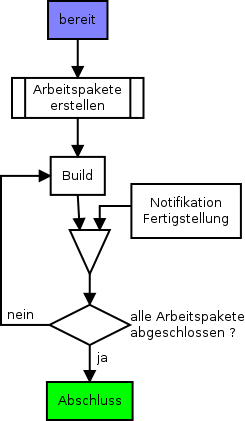
\includegraphics[height=4in]{imageinput/lebenszyklus-auftrag-abarbeitung.png}
  \caption{Auftragsannahme: Flussdiagramm}
\end{figure}

\subsubsection{Auftragsvorbereitung}

In der Auftragsvorbereitung werden Details aus dem Projekt zum Auftrag hinzugefügt.
Die vordefinierten Build-Achsen werden vom Projekt übertragen.
Dies stell sicher, dass der Aufrag und sein Umfang eindeutig bestimmt sind,
bevor mit der Erstellung von Arbeitspaketen begonnen wird.


\subsubsection{Bereitstellung von Arbeitspaketen}

Das Bereitstellen von Arbeitspaketen stellt den Anfang der eigentliche Arbeitsphase dar.
Entsprechend der Werte der Build-Achsen des Auftrages, werden nun die Arbeitspakete generiert,
wobei jedes Arbeitspaket eine der Wertekombinationen darstellt.
Nachdem alle Arbeitspakete erstellt sind, ist die Bearbeitung des Auftrages an sich abgeschlossen.

\subsubsection{Abschluss von Aufträgen}

Der Abschluss eines Auftrages ist ein Ereignis, welches Impliziert werden kann.
In im zu entwickelnden System wird der Abschluss eines Auftrages definiert,
als der Zustand der Eintritt, wenn alle Arbeitspakete eines Auftrages
einen finalen Zustand erreichen.

Dies Vereinfacht die Behandlung des Auftragsabschlusses,
da man nicht nach Abschluss von Arbeitspaketen weitere Operationen durchführen muss,
um den eventuellen Abschluss festzustellen.

\subsection{Zuteilung/Abarbeitung von Arbeitspaketen}


\subsubsection{Lebenszyklus eines Arbeitspaketes}


\begin{figure}[ht] 
  \centering
  \label{fig:lebenszyklus-arbeitspaket}
  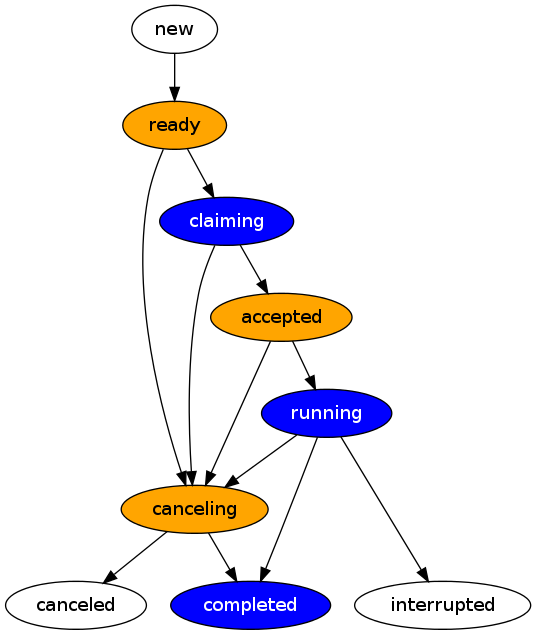
\includegraphics[height=4.5in]{imageinput/lebenszyklus-arbeitspaket.png}
  \caption{Lebenszyklus eines Arbeitspaketes bei Ausschreibungen}
\end{figure}


\subsubsection{Vorbereitung Abarbeitung}

\subsubsection{Zuteilung}


\subsubsection{Abschluss Abarbeitung}

Ist die Bearbeitung der einzelnen Schritte eines Arbeitspaketes abgeschlossen,
so muss das Resultat zusammen

- ende der arbeisschritte
- zusammenfassung resultat
- endscheidung fehlschlag oder nucht


\subsection{Überblick Methoden der Zuteilung von Arbeitspaketen}

Diese Sektion beschäftigt sich mit der Zuteilung von Arbeitspaketen.
Grundsätzlich gibt es 2 Möglichkeiten dies zu bewerkstelligen.
Es muss festgestellt werden, welche Methode besser geeignet ist.

\subsubsection{Melde-verfahren}
% MOAR
Beim Melde-verfahren teilt der Arbeiter nur seinen Arbeitwunsch mit.
Anschließend wartet er darauf, dass dieser Erfüllt wird.
Dabei liegt die Logik der Zuteilung komplett beim Manager,
er muss also über das Wissen verfügen, welcher Arbeiter in der Lage ist welche Arbeitspakete zu bearbeiten.

\begin{figure}[ht] 
  \label{fig:auftrag-zuteilung-token}
  \begin{sequencediagram}
      \newinst{worker}{:Worker}
      \newinst[1]{manager}{:Manager}
      \mess{worker}{token <spec>}{manager}
      \mess{manager}{work <spec>}{worker}
      \mess{worker}{result}{manager}
  \end{sequencediagram}
  \caption{Auftragszuteilung: Tokenbasiert}
\end{figure}

Vorteil des Verfahrens ist, das die Zuteilung ein eindeutiger Prozess ist.
Jedoch benötigt der Manager genaues wissen über die Arbeiter,
um seiner Aufgabe gerecht zu werden.

\subsubsection{Ausschreibungsverfahren}

Beim Ausschreibe-verfahren teilt der Manager die offenen Arbeitspakete mit.
Anschließend können Arbeiter einen Anspruch auf diese Anmelden.
Sie treten dabei in Konkurrenz.
Der Manager entscheidet dann, welcher Arbeiter welches Arbeitspaket bearbeiten darf.
%MOAR

Dies erlaubt Wesentlich autonomere Arbeiter,
sie sind nun in der Lage frei zu entscheiden,
welche der verfügbaren Aufträge sie bearbeiten wollen.
Der Manager ist auch Vereinfacht,
da er nur noch die Entscheidung für den Zuschlag treffen muss.
es ist nicht notwendig spezielles Wissen über die Arbeiter zu haben. 


\begin{figure}[ht] 
  \label{fig:auftrag-zuteilung-claim}
  \begin{sequencediagram}
      \newinst{workera}{:Worker A}
      \newinst[1]{manager}{:Manager}
      \newinst[1]{workerb}{:Worker B}
      \mess[1]{manager}{availiable}{workera}
      \prelevel
      \prelevel
      \mess[1]{manager}{availiable}{workerb}

      \mess[1]{workera}{claim}{manager}
      \prelevel
      \prelevel
      \mess[2]{workerb}{claim}{manager}
      %XXX: better call?
      %\prelevel
      %\prelevel
      %\begin{call}{manager}{approve}{manager}{workera}
      %\end{call}
      \mess{manager}{approve A}{workera}
      \prelevel
      \mess{manager}{approve A}{workerb}
  \end{sequencediagram}
  \caption{Auftragszuteilung: Ausschreibungsbasiert}
\end{figure}

\subsubsection{Auswahl}

Das Ausschreibungsverfahren zeigt sich im Vergleich zum Melde-verfahren
wesentlich flexibler.
Die Möglichkeit Detailkenntnisse über die Fähigkeiten eines Arbeiter nur
beim Arbeiter zu belassen, sorgt dafür, das Arbeiter wesentlich autonomer sind.
Dies hat zur Folge, dass der Zuteilungs-algorithmus wesentlich vereinfacht wird.
Da für ihn nun unerheblich ist, er den Zuschlag bekommt.
Das Ergebnis wird das gleiche sein.

\subsection{Abarbeitung von Arbeitspaketen}

Bei der Abarbeitung von Arbeitspaketen geht es darum die einzelnen Arbeitsschritte
der reihe nach linear abzuarbeiten.
es 

\subsubsection{Arbeitsschritte}


\begin{figure}[ht] 
  \centering
  \label{fig:lebenszyklus-arbeitsschritt}
  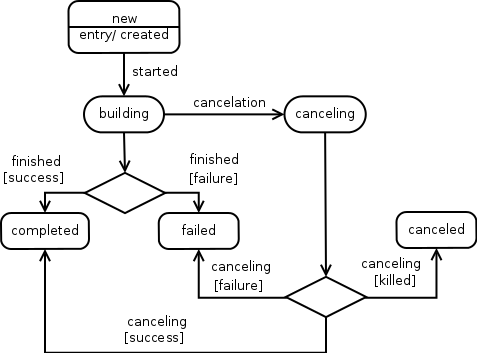
\includegraphics[height=3.4in]{imageinput/lebenszyklus-arbeitsschritt.png}
  \caption{Stategraph eines Arbeitschrittes}
\end{figure}

\begin{verbatim}
- kill wird in der impl nicht betrachtet

\end{verbatim}


\subsubsection{Datensammlung zur Laufzeit}

\begin{verbatim}
- sinn/echtzeit?

- beispielhaft
    - STDOUT/ERR
    - exakte testresultate/reports
\end{verbatim}



\subsubsection{Datensammlung nach Abschluss eines Schrittes}

Datensammlung nach dem Abschluss eines Arbeitsschritts,
Umfasst in der Regel verschiedenste Dateiformate.
Diese werden aus den verschiedensten Gründen generiert.
Üblich sind Test-Resultate, Logdateien, Build-Resultate und Archive.

Die Abbildung dieser Datensammlung kann dabei auf 2 Arten geschehen,

\begin{enumerate}
    \item als Teil des Schrittes
    \item als eigene Art von Schritt
\end{enumerate}

Die Abbildung als eigene Art von Arbeitsschritt,
hat einige Vorteile, da sie die Zuständigkeit vom reinen Arbeitsschritt
und dem Daten-sammeln sauber trennt.

Dies macht die Werkzeuge zur Datensammlung wesentlich einfacher.
Anstatt sie in jeden Schritt integrieren zu müssen,
kann einfach nach dem Schritt angewendet werden.


\subsubsection{Abschluss von Arbeitsschritten}

- returncodes
- fehler

\section{Besondere Ansätze zur Datenbank-Interaktion}

%XXX: http://dbmsmusings.blogspot.de/2010/04/problems-with-cap-and-yahoos-little.html


\subsection{CAP Abdeckung}

Wie bereits in Sektion~\ref{sec:base:cap} erwähnt,
ist es immer nur möglich 2 der 3 Aspekte des CAP Theorems abzudecken.

Jedoch ist es durchaus legitim für verschiedene Teile
einer verteilten Applikation unterschiedliche Bereiche abzudecken.
Sobald genau definiert ist, für welche Daten in welchem Kontext welche Eigenschaften benötigt werden,
kann ein konsistentes Modell geschaffen werden.

Wichtig ist bei dieser Betrachtung, dass die unterschiedlichen Komponenten des Entwickelten CI-Systems
nicht zwingend eine direkte Konsistenz-Bindung untereinander benötigen.
Wichtig ist nur, die Konsistenz zwischen einer Komponente
und dem Datenbank-knoten, mit dem sie Kommuniziert.

Das Haupt-system, in dem alle Komponenten in Kommunikation stehen,
%XXX: s1?
soll nach Systemanforderung \textbf{S1} immer verfügbar sein und somit einen Teil-Ausfall  verkraften.
Somit kommt für die Kommunikation zwischen Komponenten nur das Modell \textbf{A-P} in Frage
(was Verfügbar und Partitionstolerant bedeutet).

Die Anbindung einzelner Komponenten and ihre Datenbank-knoten, hat jedoch andere Anforderungen.
Da eine direkte Anbindung and die Datenbank für das Funktionieren einer Komponente unabdingbar ist,
kann in diesem Fall nur das Modell \textbf{C-A} zum Einsatz kommen.


%XXX: http://www.infoq.com/articles/cap-twelve-years-later-how-the-rules-have-changed


\subsection{Status-Maschinen zur Wahrung der Konsistenz}

%XXX: Literatur
% http://blog.incubaid.com/2012/10/25/caulking-your-distributed-algorithm-implementation/
\nocite{statechart}

Statusmaschienen sind ein allgemein bekanntes Werkzeug,
um den den Ablauf eines komplexen Programms zu beschreiben oder zu erklären.
In der Regel wird dazu ein sog. StatusGraph verwendet.
Dieser ist ein Gerichteter Graph der die Zustände und Zustandsänderungen eines Systems beschreibt.

Wie bereits in Abbildung \ref{fig:lebenszyklus-arbeitspaket} gezeigt,
stellt der Lebenszyklus eines Arbeitspaketes einen solchen Statusgraph dar.
Als Besonderheit ist er sogar frei von Zyklen.
Dadurch ist es unmöglich den gleichen Status noch einmal zu erreichen.

Bindet man Zusätzlich noch die Transitionen an bearbeitende Knoten (Agenten außerhalb der Datenbank),
so ist es auch bei einer Partitionierung der Datenbank eine Konsistenz der Gesamtsystems gewährleistet.

%XXX: moar?


Mit dem dem Eingang und der Abarbeitung von Aufträgen verhält es sich ähnlich,
jedoch ist der Graph dort Wesentlich einfacher.
Die Abbildungen \ref{fig:lebenszyklus-auftrag-eingang} und \ref{fig:lebenszyklus-auftrag-abarbeitung} zeigen den groben Ablauf.
Der Wechselpunkt zwischen Eingang und Abarbeitung ist die der Validation angeschlossene Markierung zur Bereitschaft.
Da es nur diesen einen Punkt des Austausches gibt, ist die Wahrung der Konsistenz des Auftrages denkbar einfach,
Mit der Bereitschaft, wird die Verantwortung vom Eingang zur Abarbeitung übertragen.

\subsection{Abbildung des Verteilten Systems auf Datenbanken}

Die Abbildung eines verteilten Systems auf eine Datenbank,
hat einige überaus erfreuliche Nebeneffekte.

Im Client-Server System müssen der Client und Server extra Nachrichten Austauschen, um das gleiche Bild der Welt zu bekommen, wobei jedes System eine eigene Version des Zustandes hat.
Beim Datenbank-basierten System ist der Status jedoch in der Datenbank und
die einzelnen Komponenten des Systems müssen somit nicht weiter eigene Kopien vorhalten.

Eine Änderung des Status wird nun durch eine Änderung in der Datenbank zum Ausdruck gebracht.
Sobald die Änderung in die Datenbank eingebracht ist,
ist der Vorgang des Übermittelns für die sendende Komponente abgeschlossen.
Sie muss nicht wie bisher auf eine Rückantwort warten.

\subsection{Auftragsverteilung}

\section{Logisches Gesamtkonzept}
\subsection{Eingang}
\subsection{Management}
\subsection{Arbeiter}

\section{Arbeitsschritte und der Kontext ihrer Ausführung}

\subsection{Überblick und grundlegender Ablauf}

\begin{figure}[!ht]
  \centering
  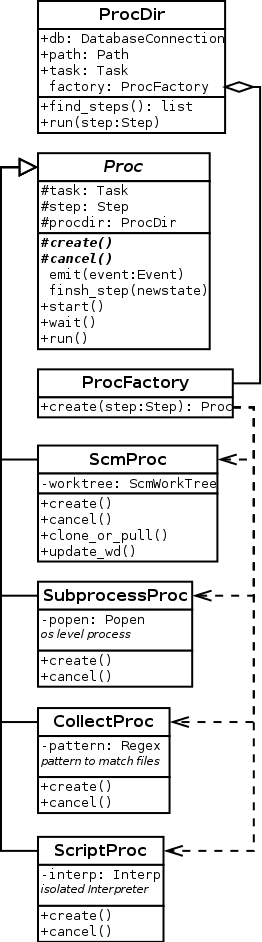
\includegraphics[height=0.8\textheight]{imageinput/klassen-arten-arbeitsschritt.png}
  \caption{Arten und Ablauf von Arbeitsschritten}
  \label{fig:klassen-arten-arbeitsschritt}
\end{figure}

Wie man auf der Grafik~\ref{fig:klassen-arten-arbeitsschritt} gut erkennen kann,
bildet das Arbeitsverzeichniss (ProcDir) die Basis
für die Durchführung der Arbeitsschritte eines Auftrages.

Es bindet alle Operationen, die notwendig sind,
um die Kontrolldaten (Steps, siehe Fig~\ref{fig:datenstrukturen})
aus der Datenbank zu laden und diese dann an Ausführende Objekte zu binden (Proc).

Der Lebenszyklus eines ``Proc'' Objektes wird dabei vom zugehörigen Procdir verwaltet.
das Proc Objekt sollte nur innerhalb der Methode run existieren.
\lstset{language=python}
\begin{lstlisting}
#pseudocode
class ProcDir:
    def __init__(self, procmaker):
        self.procmaker = procmaker
    def run(self, step):
        proc = self.procmaker.create(step)
        return proc.run()
\end{lstlisting}

%XXX: More

\subsection{Prozess Schritte}

Die Aufgabe eines Prozessschrittes ist es,
einen Programm mit vorgegebenen Parametern auszuführen.
Dies ist auch der Grund, warum der ``ProcessProc'' Datentyp einen
Prozess-Handle enthält.

Dabei Fallen zur Laufzeit sammelbare Daten wie z.B. Text auf den Standard Eingabe-/Ausgabe Datenströmen an.
Außerdem verändern sich statistische Informationen über den Prozess wie Speicher-verbrauch, IO-Last, u.a.


\subsection{Skript Schritte}

Skript-Schritte unterscheiden sich von Prozess-Schritten in der Hinsicht,
dass sie kein Programm an sich, sondern ein Skript ausführen.
Daher können sie in die Lage versetzt werden,
weitere Laufzeit-Daten zur Verfügung zu stellen


\subsection{Quellcode Management Schritte}

Quellcode Management Schritte behandeln die Interaktion mit dem SCM.
Es wird, wenn notwendig ein Arbeitsverzeichniss erstellt.
Danach gibt es mehrere Grundlegende Operationen, die durchgeführt werden können.

\begin{description}
    \dhitem[Eingang von Historie]
        bringt die lokale Historie auf den aktuellen Stand, ``pull'' genannt
    \dhitem[Aktualisierung des Arbeitsverzeichniss]
        aktualisiert die Dateien im Arbeitsverzeichniss
        auf eine gewünschte Version
    \dhitem[Anwendung von Patches]
        wendet Patches auf das aktuelle Arbeitsverzeichniss an
\end{description}


\subsection{Datensammlungs Schritte}

Datensammlung-schritte haben die Aufgabe,
bei vorhergehenden Schritten entstandene Dateien 
in die Datenbank zu überführen.
Die Grundfunktion pflegt dabei nur den Inhalt der Datei ein.
Laufzeit-Daten dieses Schritts sind die gefundenen Dateien.

Dabei wird das Regexmuster ``pattern'' verwendet, um festzustellen,
ob eine Datei im Arbeitsverzeichniss, zur Menge der gewünschten Dateien gehört.

Erweiterte Versionen dieser Schritt-Art, könnten zusätzliche Funktionen,
wie z.b. Einpflegen von Testergebnissen aus JunitXML Dateien in die Datenbank,
übernehmen

\section{Erweiterungen}

\subsection{Analyse Test-Resultate}

Bei der Analyse von Test-Resultaten ist das Ziel Veränderungen in Verschiedenen Umgebungen feststellen zu können.
Ziel ist es dabei Vorwiegend Unterschiede zwischen verschiedenen Arbeitspaketen und Aufträgen festzustellen. Unterschiede zwischen Zeitlich aufeinander Folgenden Aufträgen oder Arbeitspaketen, welche verschiedene Plattformen, Entwickler-zweige oder Konfigurationen betrachten, geben Aufschluss über Entwicklung und Zustand des Projektes.

Da ein großer Teil dieser Erweiterung zur Benutzeroberfläche gehört,
werden hier nur die unterstützenden Algorithmen und Datenstrukturen betrachtet.
Um überhaupt Vergleiche anstellen zu können, muss zuerst die Vergleichs-menge bestimmt werden. Dabei erscheint die Menge an Test-Resultaten je Arbeitsschritt am geeignetsten. Im Gegensatz zur Menge an Test-Resultaten je Auftrag,
ist in diesem Fall für jede Konfiguration ein Set an Resultaten verfügbar.

Um Testresultate abzulegen, erscheint es sinnvoll eine weitere Art an Datenstruktur einzuführen.
Diese sollte wie die Bereits definierten ``Events'' aufgebaut sein,
jedoch soll es möglich sein, diese aus einem Prozess der den Testvorgang verwaltet,
anzulegen. Zudem sollen sie an das Arbeitspaket und nicht an den Arbeitsschritt gebunden sein.

Für die Vergleiche ist es nun Notwendig,
Unterschiede zwischen 2 oder mehr Mengen an Testresultaten zu bestimmen.
Eine recht einfache Methode ist dabei die Mengen-Differenz,
Nimmt man für die Testresultate eine Werte-menge mit der Struktur \{ $Testname \rightarrow Resultat$ \} als Basis,
so ist es leicht einen passenden Überblick aufzubauen.

Die Datenstruktur der Resultate, für Vergleiche zischen N Resultatmengen
ist dabei eine Zuordnung von
$\{ Testname \rightarrow ( Resultat_{1},\ldots,Resultat_{N})\}$
Wobei idr. nur die Elemente interessant sind,
deren Resultat-menge Unterschiede und/oder Fehlschläge aufweist.
Ein gutes Beispiel für die Darstellung eines solchen Resultates
stellt der Testresultatüberblick des Pypy Projektes \cite{pypy:overview} dar.

Die Art und Weise wie die Mengen an Test-resultaten für die Vergleiche ausgewählt werden sollen, werden in dieser Arbeit nicht betrachtet,
da dies vorwiegend ein Problem der Benutzeroberfläche ist.

\subsection{Analyse Verhalten eines Programms}

Bei der Erweiterung zur Analyse des Verhaltens eines Programms,
geht es darum das Verhalten eines Programms
in verschiedenen Konfigurationen zu testen.
Als Programm wurde dabei ein Skript gewählt,
welches einen genetischen Algorithmus umsetzt.

Im willkürlich gewählten Beispiel ist dies ein Programm,
welches versuchen soll, eine Funktion anzunähern \cite{gen:prog}.

Die Analyse soll dazu dienen, Parameter-werte festzustellen,
die zum Erfolg des Algorithmus führen.
Bei der Betrachtung steht die Analyse der Resultate nach der Durchführung des Programms im Vordergrund,

Dabei wurden die folgenden Konfigurations-achsen für Parameter gewählt.

\begin{description}
    \item[generations] Menge der Generationen
    \item[population] Größe der Population
    \item[height-weight] Bewertungsgewicht für die Höhe des Baumes welcher die angenäherte Funktion zum Ausdruck bringt
\end{description}

Die Achsen ``generations'' und ``population'' sind dabei ein exponentiell wachsender Wertebereich zwischen 20 und 5000.
Die Achse ``height-weight'' hingegen wurde im Bereich zwischen -2 und 2 gewählt,
wobei viele Werte im Bereich $ 0<abs(x)<1$ liegen.

Die Wahl der Achsen und ihrer Parameter ist willkürlich als Teil eines ersten Tests entstanden.
Weitere Parameter und Achsenkonfigurationen sind denkbar.
Das Analysewerkzeug soll zeigen welchen Einfluss die Parameter haben.

Um dies zu zeigen, ist es notwendig die Resultate
eines Konfigurierten Durchlaufes (Auftrag) Zusammenzufassen.
Die Resultate jedes einzelnen Auftrages sind dabei aus der Standardausgabe
des Programms zu entnehmen.

Für jedes Arbeitspaket eines Auftrages sind also Parameter-werte und Ergebnis zusammenzufassen.
Anschließend können die Daten in Graphen dargestellt werden.


\section{Benutzeroberfläche}

Da die Benutzeroberfläche für den Prototypen nicht zwingend notwendig,
wird darauf verzichtet, mehr als nur simple Werkzeuge zur Verfügung zu stellen.
Wichtig ist dabei, dass vorgefertigte Testdaten in die Datenbank eingegeben werden können.


\section{Zusammenfassung}

was kommt
was kommt nicht
